\documentclass[a4paper]{article}

\usepackage[utf8x]{inputenc}    
\usepackage[T1]{fontenc}
\usepackage[spanish]{babel}
\usepackage{multicol}

\usepackage{wrapfig}
\usepackage{graphicx}

\usepackage{bm}
\usepackage{amsxtra} 
\usepackage{amssymb}% to get the \mathbb alphabet
\usepackage{amsmath}

\usepackage[spanish]{cleveref}


\usepackage[box,completemulti,separateanswersheet]{automultiplechoice}    
\def\AMCformQuestion#1{\vspace{\AMCformVSpace}\par {\sc Pregunta #1:} }    
\def\AMCbeginQuestion#1#2{\par\noindent{\bf Pregunta #1}#2\hspace*{1em}}
\def\AMCcleardoublepage{\ifodd\thepage\clearpage\mbox{}\fi\clearpage}

\begin{document}

\AMCrandomseed{1237893}

%%%%%%%%%%%%%%%%%%%%%%%%%%%%%%%%%%%%%%%%%%%%%%%%%%%%%%%%%%%%%%%%%%%%%%%%%%%%%
\element{test1}{
\begin{question}{p1}
El valor del desplazamiento en direcci\'on $x$ del punto I vale aprox:
\begin{multicols}{2}
\begin{choices}
	\correctchoice{$1.5$ cm}
	\wrongchoice{$11.7$ cm}
	\wrongchoice{$0.63$ cm}
	\wrongchoice{$5.9$ cm}
\end{choices}
\end{multicols}
\end{question}
}
%%%%%%%%%%%%%%%%%%%%%%%%%%%%%%%%%%%%%%%%%%%%%%%%%%%%%%%%%%%%%%%%%%%%%%%%%%%%%
%\element{test1}{
%\begin{question}{p2}
%El valor del giro en direcci\'on $z$ del apoyo de la primera columna vale aprox:
%\begin{multicols}{2}
%\begin{choices}
%	\correctchoice{$-4.0\cdot10^{-4}$ rad}
%	\wrongchoice{$-1.1\cdot10^{-4}$ rad}
%	\wrongchoice{$-5.6\cdot10^{-3}$ rad}
%	\wrongchoice{$2.1\cdot10^{-4}$ rad}
%\end{choices}
%\end{multicols}
%\end{question}
%}
%%%%%%%%%%%%%%%%%%%%%%%%%%%%%%%%%%%%%%%%%%%%%%%%%%%%%%%%%%%%%%%%%%%%%%%%%%%%%
\element{test1}{
\begin{question}{p3}
El valor de la máxima flecha vertical en el vano CF vale aprox.:
\begin{multicols}{2}
\begin{choices}
	\correctchoice{$3.4$ mm}
	\wrongchoice{$2.1$ mm}
	\wrongchoice{$0.91$ mm}
	\wrongchoice{$1.7$ mm}
\end{choices}
\end{multicols}
\end{question}
}
%%%%%%%%%%%%%%%%%%%%%%%%%%%%%%%%%%%%%%%%%%%%%%%%%%%%%%%%%%%%%%%%%%%%%%%%%%%%%
\element{test1}{
\begin{question}{p4}
El valor máximo de la componente vertical de la reacción en el apoyo de la columna central vale aprox.:
\begin{multicols}{2}
\begin{choices}
	\correctchoice{$620.9$ kN}
	\wrongchoice{$ 120.4$ kN}
	\wrongchoice{$ 53.1$ kN}
	\wrongchoice{$ 8001.3$ kN}
\end{choices}
\end{multicols}
\end{question}
}
%%%%%%%%%%%%%%%%%%%%%%%%%%%%%%%%%%%%%%%%%%%%%%%%%%%%%%%%%%%%%%%%%%%%%%%%%%%%%
\element{test1}{
\begin{question}{p5}
El valor del momento máximo en direcci\'on $z$ en el centro del vano FI, en valor absoluto, vale aprox.:
\begin{multicols}{2}
\begin{choices}
	\correctchoice{$ 83.6$ kN m}
	\wrongchoice{$34.1$ kN m}
	\wrongchoice{$51.9$ kN m}
	\wrongchoice{$104.9$ kN m}
\end{choices}
\end{multicols}
\end{question}
}
%%%%%%%%%%%%%%%%%%%%%%%%%%%%%%%%%%%%%%%%%%%%%%%%%%%%%%%%%%%%%%%%%%%%%%%%%%%%%
%\element{test1}{
%\begin{question}{p6}
%El valor del cortante máximo en el vano FI, en valor absoluto, vale aprox.:
%\begin{multicols}{2}
%\begin{choices}
%	\correctchoice{$ 46$ kN}
%	\wrongchoice{$ 21 $ kN}
%	\wrongchoice{$  12$ kN}
%	\wrongchoice{$  108$ kN}
%\end{choices}
%\end{multicols}
%\end{question}
%}
%%%%%%%%%%%%%%%%%%%%%%%%%%%%%%%%%%%%%%%%%%%%%%%%%%%%%%%%%%%%%%%%%%%%%%%%%%%%% 
\element{test1}{
\begin{question}{p7}
El valor del axil máximo en el vano FI, en valor absoluto, vale aprox.:
\begin{multicols}{2}
\begin{choices}
	\correctchoice{$ 359$ kN}
	\wrongchoice{$ 30 $ kN}
	\wrongchoice{$  1140$ kN}
	\wrongchoice{$  880$ kN}
\end{choices}
\end{multicols}
\end{question}
}
%%%%%%%%%%%%%%%%%%%%%%%%%%%%%%%%%%%%%%%%%%%%%%%%%%%%%%%%%%%%%%%%%%%%%%%%%%%%%
%\element{test1}{
%\begin{question}{p8}
%En la formulación de vigas de Euler-Bernoulli, el esfuerzo cortante:
%%\begin{multicols}{2}
%\begin{choices}
%       \correctchoice{Se calcula con la ecuación de equilibrio de momentos}
%        \wrongchoice{Se calcula a partir de la deformación angular $\gamma_{xz}$}
%        \wrongchoice{Por hipótesis, se toma iguaL a $0$}
%        \wrongchoice{Ninguna de las otras respuestas es correcta}
%\end{choices}
%%\end{multicols}
%\end{question}
%}
%%%%%%%%%%%%%%%%%%%%%%%%%%%%%%%%%%%%%%%%%%%%%%%%%%%%%%%%%%%%%%%%%%%%%%%%%%%%%%
%\element{test1}{
%\begin{question}{p9}
%Los elementos finitos de viga de Bernoulli \ldots
%%\begin{multicols}{2}
%\begin{choices}
%        \correctchoice{Incorporan la hipótesis de que las secciones normales se mantienen indeformables, planas y normales a la directriz}
%        \wrongchoice{Incorporan la hipótesis de que las secciones normales se mantienen indeformables, planas pero no necesariamente normales a la directriz}
%        \wrongchoice{Incorporan la hipótesis de que las secciones normales se mantienen planas y normales a la directriz, pero pueden deformarse en dirección transversal por las cargas aplicadas}
%        \wrongchoice{Las funciones de interpolación de los elementos finitos \(N_a(x)\) pueden ser lineales}
%\end{choices}
%%\end{multicols}
%\end{question}
%}
%%%%%%%%%%%%%%%%%%%%%%%%%%%%%%%%%%%%%%%%%%%%%%%%%%%%%%%%%%%%%%%%%%%%%%%%%%%%%%
%\element{test1}{
%\begin{question}{p10}
%Los elementos finitos de viga de Timoshenko \ldots
%%\begin{multicols}{2}
%\begin{choices}
%        \correctchoice{Incorporan deformación por cortante de la viga}
%        \wrongchoice{Incorporan la hipótesis de que las secciones normales se mantienen indeformables, planas y normales a la directriz}
%        \wrongchoice{Para vigas muy poco esbeltas pueden producir bloqueo de la solución numérica}
%        \wrongchoice{Las funciones de interpolación de los elementos finitos \(N_a(x)\) deben ser al menos cúbicas}
%\end{choices}
%%\end{multicols}
%\end{question}
%}
%%%%%%%%%%%%%%%%%%%%%%%%%%%%%%%%%%%%%%%%%%%%%

\scoringDefaultS{b=1,m=-1/(N-1)}

\onecopy{10}{    

%%% beginning of the test sheet header:    

\noindent{\large\bf Método de los Elementos Finitos  \hfill MUECYM \hfill FINAL ORD. \# Ej. 2}
\begin{center}
%\vspace*{.1cm}
%Se atribuirá puntuación negativa a las respuestas incorrectas.\\
\vspace*{.1cm}
20 ene 2025. \hspace{7cm} Tiempo: 45 minutos.\\


\end{center}

\vspace{1ex}

El pórtico de dos vanos mostrado en la figura es de hormigón armado con módulo de elasticidad $E=32$ GPa, coeficiente de Poisson $\nu=0.20$, y densidad de masa  $\rho=2548.42$ kg/m$^3$. Las secciones de las vigas son de $0.30$ m $\times$ $0.60$ m (base y altura), y las columnas tienen sección cuadrada de $0.40$ m de lado. Las cargas actuantes sobre la estructura son el peso propio del pórtico, dos cargas puntuales verticales (en J y K), una carga puntual horizontal (en C) y una carga distribuida (sobre las vigas). Los apoyos A, D y G se consideran perfectamente empotrados. Los letras B, J, E, K y H indican la mitad de cada uno de los respectivos elementos estructurales.

Se pide realizar un modelo de vigas con elementos tipo B23, tamaño de elementos $0.5$ m y responder las preguntas del cuestionario.

Las longitudes del pórtico son tal como sigue: $l_{1}= 6$ m, $l_{2}= 5$ m, $l_{3}= 3$ m, $l_{4}$ y $l_{5}= 5$ m. Las cargas son $V_{1}= 70$ kN, $V_{2}= 50$ kN, $H_{1}= 488.40$ kN, y $q_{1}= 100$ kN/m. Las dimensiones de los elementos estructurales son $a= 0.40$ m, $b= 0.30$ m y $c= 0.60$ m.
\\
\begin{center}
	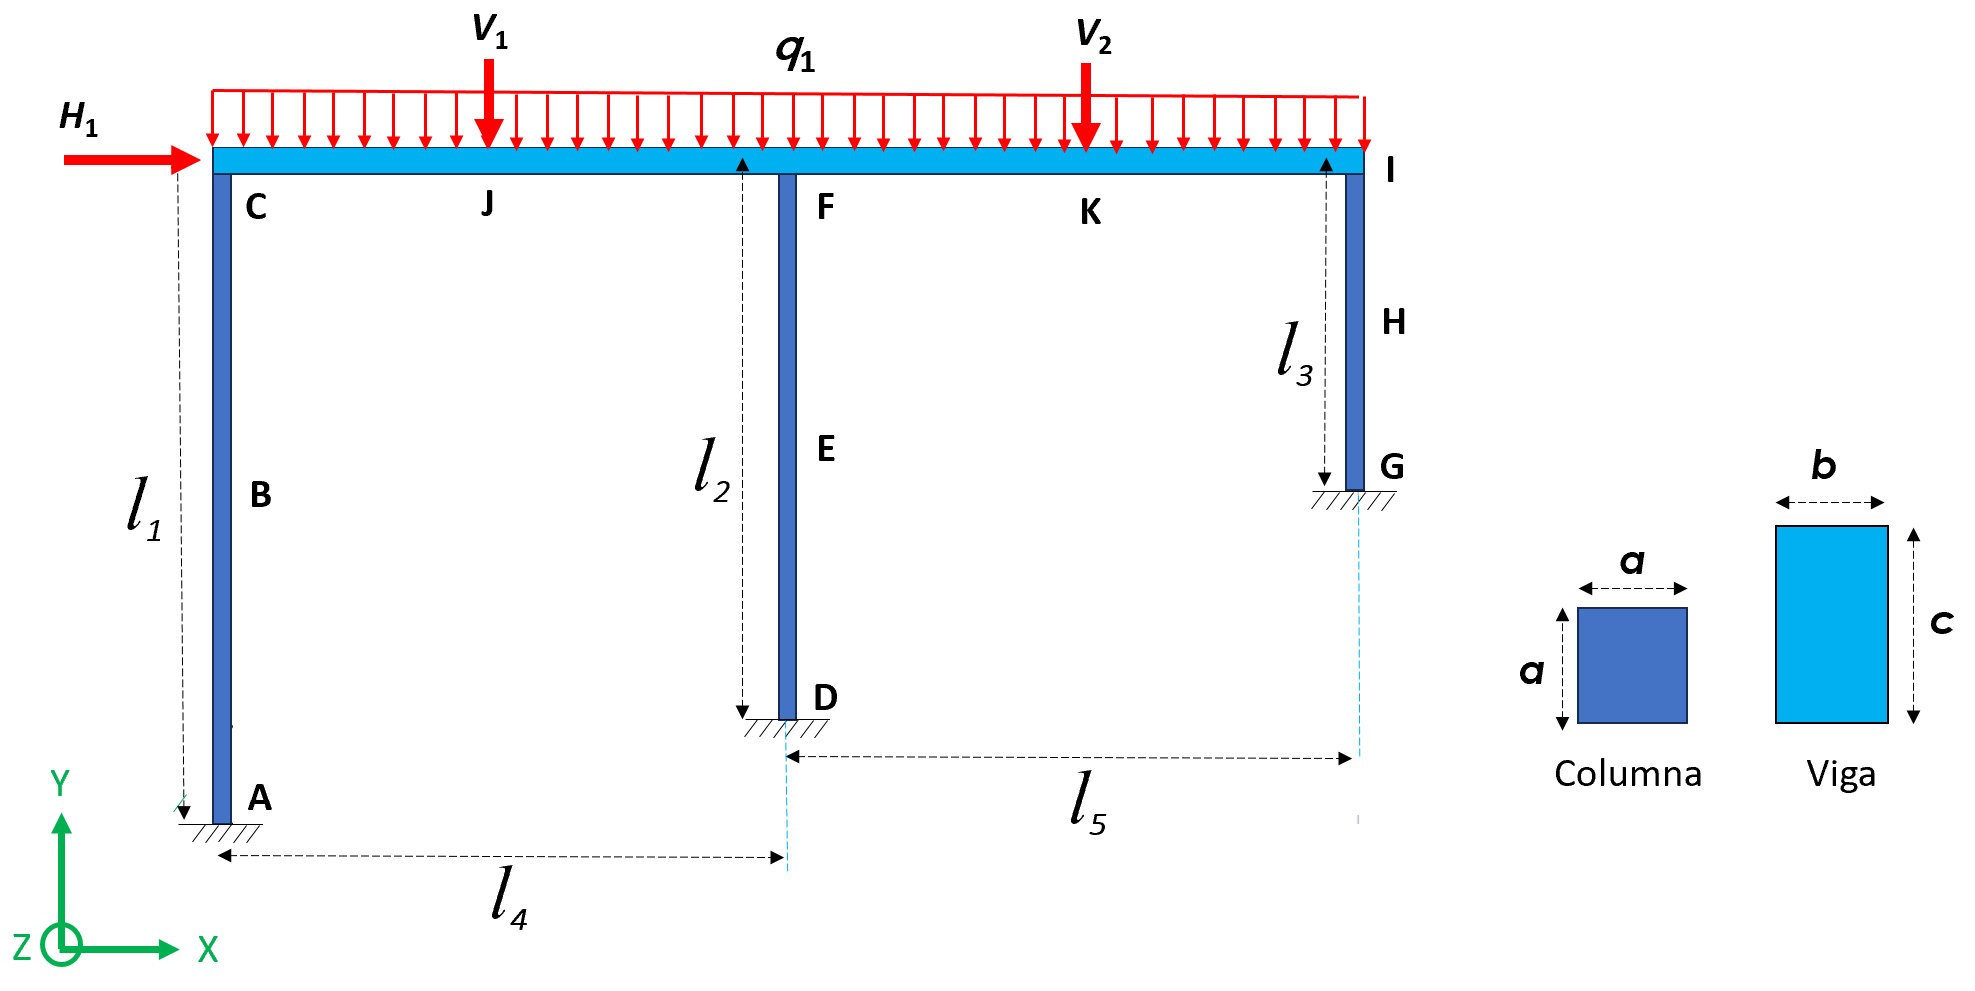
\includegraphics[width=1.05\textwidth]{figuraNT2023}
\end{center}


\hrulefill
\vspace{4mm}

%%% end of the header

\shufflegroup{test1}
\insertgroup{test1}

%\AMCcleardoublepage    
\clearpage

\AMCformBegin    

%%% beginning of the answer sheet header

\noindent\AMCcode{nummat}{2}\hspace*{\fill}
\begin{minipage}{.7\linewidth}
$\longleftarrow{}$ Escriba su número de matrícula marcando los dígitos
en los recuadros (con ceros a la izquierda si el número es de menos de dos dígitos) y el nombre y apellidos debajo.

\vspace{3ex}

\namefield{\fbox{
   \begin{minipage}{.9\linewidth}
     Apellidos, Nombre:

     \vspace*{.5cm}\dotfill
     \vspace*{1mm}
   \end{minipage}
 }}
\end{minipage}

\begin{center}
 \bf\em Debe dar las respuestas exclusivamente en esta hoja (las respuestas en las demás hojas no serán tenidas en cuenta).
\end{center}

%%% end of the answer sheet header


\AMCform    

\AMCcleardoublepage    

}  

\end{document}
